\section{NEMD Set-up}
\label{sec:setup}

In this work, non-equilibrium molecular dynamics (NEMD) simulations are performed using the 
LAMMPS~\cite{Plimpton:2007} software package.
Essentially, a temperature gradient is applied by means of Langevin thermostats located
at $L$/4 and $3L$/4 in a silicon bar of length, $L$ 
as shown using a schematic in Figure~\ref{fig:setup}. 

\begin{figure}[htbp]
\begin{center}
\begin{tabular}{cc}
  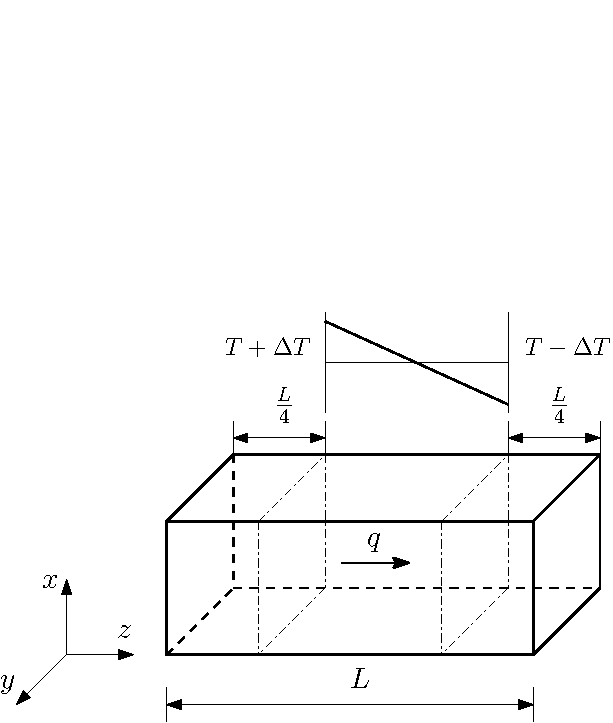
\includegraphics[width=0.48\textwidth]{schematic}
  &
  \hspace{3mm}
  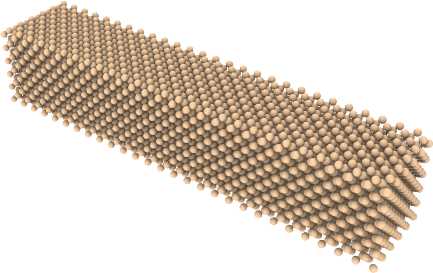
\includegraphics[width=0.40\textwidth]{Sibar_05}
  \\ (a) & (b)
  \end{tabular}
\caption{(a) Schematic illustration of the set-up for evaluating thermal conductivity of Si using NEMD. (b) 
Arrangement of Si atoms prior to the application of temperature gradient.}
\label{fig:setup}
\end{center}
\end{figure}

The set of
inputs to LAMMPS is provided below in Table~\ref{tab:input}. Note that specific values for the length of the bar
and the applied temperature gradient are not provided since we investigate thermal conductivity trends for a range of 
values of the two parameters as discussed later in Section~\ref{sec:response}. A careful analysis focused on
minimizing temperature fluctuations during different stages of the simulation was performed to optimize for the
choice of height and width of the bar as well as the duration of the simulation. 

\begin{table}[htbp]
\begin{center}
\begin{tabular}{|c||c|}
\hline
Lattice Constant, $a$ ($\angstrom$) & 5.43 \\ \hline
Width, Height ($\angstrom$) & 22$a$ \\ \hline
$\Delta t$  (ps) & 0.0005 \\ \hline
Simulation Run Length (ps) & 320 \\ \hline
Boundary Condition & Periodic \\ \hline
Lattice Structure & Diamond \\ \hline
Inter-atomic Potential & Stillinger-Weber \\ 
\hline
\end{tabular}
\end{center}
\label{tab:input}
\caption{Set of inputs for the NEMD simulation to estimate thermal conductivity in a Si bar using LAMMPS.}
\end{table}

The NEMD simulation has three stages associated with it as illustrated below in the flow diagram. In the
first stage, the NVT ensemble equilibrates the system to a specified bulk temperature, i.e., the temperature
at which thermal conductivity is to be estimated. In the second stage, the NVE ensemble equilibrates the
thermostats at their respective temperatures. It is followed by another NVE ensemble that captures the
trajectory of individual atoms and results in a steady state estimate for the thermal energy exchange between
the two thermostats. 

\begin{center}

NVT \hspace{5mm} $\rightarrow$ \hspace{5mm} NVE \hspace{5mm}
$\rightarrow$ \hspace{5mm} NVE
\\ \vspace{1mm}
\tiny \hspace{-5mm}[Equilibrate system to 300 K] \hspace{1mm} [Equilibrate thermostats] \hspace{4mm}
 [Generate Data]
\\ \vspace{1mm}

\tiny{N: Number of Atoms~~~V: Volume~~~T: Temperature~~~E: Energy}
\end{center}

The steady state exchange energy ($q$) is used in Fourier's law to estimate bulk thermal conductivity ($\kappa$)
for the Si  bar:

\be
 \kappa = \frac{q''}{\left|\frac{dT}{dz}\right|} 
\ee

\noindent where $q''$ denotes the steady state heat flux (W/m$^2$) and
$\left|\frac{dT}{dz}\right|$ denotes the magnitude of the applied 
temperature gradient along the direction of heat flow (see~Figure~\ref{fig:setup}(a)).






















